\documentclass[12pt]{article}
\usepackage{amsmath}
\usepackage{sbc-template}
\usepackage{multirow}
\usepackage{graphicx}
\usepackage{url}
\usepackage{hyperref}
\usepackage{verbatim}
\usepackage[brazil]{babel}  
\usepackage[utf8]{inputenc}
\usepackage[numbers]{natbib}

%\sloppy

\title{Aprendizagem de máquina aplicada ao reconhecimento e \\verificação de assinaturas}

\author{Daniel Elias\inst{1}, Paulo Henrique\inst{1} e \\Pedro Afonso\inst{1}}

\address{Departamento de Informática -- Instituto Federal de Educação,\\ 
	Ciência e Tecnologia de Minas Gerais (IFMG)\\ Sabará -- MG -- Brasil
	\email{\{danielias.santos, paulohenriquercs, pedroafonsouza\}@gmail.com}
}

\begin{document} 
	
	\maketitle
	
	\begin{resumo} 
		A verificação da autenticidade de assinaturas manuscritas é tarefa realizada cotidianamente em instituições financeiras e cartórios, entre outros, para comprovar a autoria de intenções e acordos em documentos de interesse. Essa analise de autenticidade quando feita por humanos, está restrita a profissionais especializados que, ainda assim, podem cometer erros. Desta forma, a automatização da atividade pode trazer benefícios, como a redução de custos e a celeridade. Associadas à essa automatização, técnicas de inteligência artificial, tal como a aprendizagem de maquina, podem ser aplicadas para minorar a ocorrência de erros. Portanto, este trabalho busca propor um sistema de verificação da autenticidade de assinaturas utilizando técnicas de aprendizagem de maquina, para verificar o desempenho, viabilidade e qualidade dos resultados esperados.
	\end{resumo}
	
	\section{Introdução}
		Assinaturas manuscritas são o meio mais utilizado, atualmente, para firmar contratos e intenções. Conforme fundamentou Freitas\textsuperscript{\cite{freitas2003}}, sistemas de gerenciamento e controle de informações, inerentes à era digital, são constantemente confrontados com este instituto arcaico, mas estabelecido, de atribuição da autenticidade de documentos, que é a assinatura manuscrita. Neste sentido, diversos são os estudos realizados para harmonizar estes dois aspectos que, em grande medida, se mostram antagônicos. Além disso, as assinaturas representam, juridicamente, a comprovação de intenções e acordos, que geram responsabilidades a seus autores. Vê-se, então, que a assinatura tem valor para o seu autor e, portanto, há o risco de fraudes.
		
		Além disso, diversos fatores subjetivos influenciam a forma das assinaturas manuscritas, tais como nacionalidade, idade, tempo, hábitos, estado psicológico ou mental e condições físicas do autor. A verificação de assinatura tem o objetivo de comprovar a autenticidade por meio de comparação, entre uma assinatura reconhecida como verdadeira e outra que esteja sob questionamento\textsuperscript{\cite{goncalves2008}}. Ainda segundo Gonçalves\textsuperscript{\cite{goncalves2008}}, os métodos de aquisição de assinaturas podem ser \textit{on-line}, por meio de \textit{hardwares} específicos (tal como mesa digitalizadora) ou \textit{off-line}, método tradicional, no qual a assinatura é disposta em papel, e aí se enquadram os sistemas automáticos de verificação.	
		
		Segundo Coetzer\textsuperscript{\cite{coetzer2006}}, os seres humanos apresentam altos índices de erros no processo de verificação de 		assinaturas. Percebe-se, então, que esta é uma tarefa árdua, atribuída a profissionais especialistas, e ainda assim está sujeita a erros. Gonçalves\textsuperscript{\cite{goncalves2008}} cita os tipos de erros cometidos, que podem ser de ``falsa rejeição'', quando uma assinatura genuína é verificada como falsa, e ``falsa aceitação'', quando uma assinatura falsa é classificada erroneamente como genuína.
		
		O intuito da verificação automática de assinaturas, em termos práticos, é prover automatização, velocidade, escalabilidade e segurança à atividade, nos mais diversos contextos aplicáveis. Desta forma, este trabalho pretende desenvolver um sistema que, por meio da aprendizagem de máquina, seja capaz de executar a verificação de assinaturas manuscritas com uma taxa de erro aceitável, em relação ao desempenho humano da tarefa.
	
	\section{Objetivo}
		Através de técnicas de aprendizado de máquina, envolvendo algoritmos de inteligencia artificial, tratamentos e aplicações de técnicas de simplificação, binarização e segmentação das imagens de assinaturas, este artigo tem como objetivo mensurar as taxas de erros e acertos de uma autenticação feita de forma automática, para verificar sua viabilidade, precisão, escalabilidade, segurança e aceitabilidade.
	
	\section{Trabalhos Relacionados}
		A fim de observar metodologias existentes na área de verificação de assinaturas que utilizam técnicas de aprendizado de máquina, foram estudados trabalhos relevantes ao assunto. Para Gonçalves\textsuperscript{\cite{goncalves2008}} os métodos \textit{on-line} e \textit{off-line} se diferem na concepção da assinatura, porém cada um tem seus prós e contras. A ideia do autor é melhorar a capacidade de análise da abordagem \textit{off-line} uma vez que é a mais utilizada.
		
		Relacionado à maneira de serem obtidas as assinaturas Freitas\textsuperscript{\cite{freitas2003}} ressalta que para se obter o reconhecimento de uma dada forma escrita é necessário estabelecer um grau de comparação entre as outras formas de treinamento afim de obter um maior grau de semelhança dos itens. Em seu outro estudo Justino\textsuperscript{\cite{justino2001}} explica que existem elementos técnicos genéticos que mitas vezes passam imperceptíveis pela análise computacional, e portanto é necessário aumentar o grau de verificação nesses quesitos. Neste trabalho são usadas essas considerações para a construção de um sistema capaz de verificar as formas escritas. 
		
		No estudo de Tebaldi\textsuperscript{\cite{tebaldi2007}}, é mostrado um exemplo de comparação de assinaturas. O modelo é feito de forma complexa, utilizando o algoritmo R-prop, que é uma vertente do \textit{back-propagation}, porém o resultado do estudo não é tão satisfatório.
		
		Talvez o mais relacionado aos processamento dos dados abordados por este objeto de estudo, o artigo de Srinivasan\textsuperscript{\cite{srinivasa2006}}, em que se utiliza a transformação em uma vetor binário dos objetos de treinamento. Também utiliza recursos matemáticos de extração relacionados ao gradiente, características estruturais, concavidade e relações de inclinação das imagens. 	
		
		O trabalho de Drott\textsuperscript{\cite{drott2015}} utilizada a comparação entre duas assinaturas e classificando-as, se são escritas por a mesma pessoa (partida) ou não (sem partida). O problema da classificação binária é então abordado com algumas alternativas para entender melhor. Primeiro por um característica de engenharia simples, em seguida, pelas técnicas de aprendizado de máquina como logística de regressão, perceptron multi-camada e, abordagem de aprendizagem profunda \textit{Deep learning} com um rede neural convolucional.
		
		Um trabalho interessante foi o de Hafemann\textsuperscript{\cite{hafemann2017}}, em que consiste no tratamento de assinaturas escritas através de dispositivos sensíveis ao toque, com um conceito de tecnologia biométrica, com um conceito de reconhecimento baseado em medições de características biológicas, como a impressão digital, rosto, íris, assinatura manuscrita, etc. Assim utiliza-se neste trabalho o aprendizado de máquina profundo \textit{Deep learning} e SVM \textit{Support Vector Machines}. 
	
	\section{Metodologia}
		\subsection{Coleta dos dados}
			Foram recolhidas diversos exemplares de assinaturas manuscritas de alunos do IFMG unidade Sabará, com o intuito de alimentar a base de dados em que serão inferidos os processamentos devidos para a utilização de dados viáveis.
		
		\subsection{Processamento da imagem}
			As imagens das assinaturas foram escaneadas através da Impressora Laser Monocromática MS811DN. Foram realizados recortes nas assinaturas de forma a estabelecer um padrão de dimensões de altura e largura para o consumo da programa ImageJ. Para determinar os recortes foi estabelecido uma dimensão para a prancheta de cada assinatura (1200x488px) feita pelo software GIMP 2.
			
			A partir da utilização do programa ImageJ, e da execução do \textit{plugin} \textit{Trainable Weka Segmentation}, se sucederam uma sequência de inferências nas imagens selecionadas, como uma binarização da imagem de assinatura em \textit{8-bits},que permite o tratamento de problemas de inclinação, fundos ruidosos, rabiscos, dados sobrescritos, dados sublinhados, e uma aplicação da técnica \textit{Thresholding}, que define automaticamente ou interativamente valores de limite inferiores e superiores, em seguida a aplicação de segmentação, que consiste em localizar automaticamente os campos relevantes do documento, ou seja, as áreas que possuem informação manuscrita a ser reconhecida, utilizando o tipo de segmentação global (quando é como único).
			
			Assim se processando recursos de interesse e plano de fundo, ou seja define-se classes de pixels, que geralmente são chamadas de "primeiro plano" e "segundo plano". Assim, foram utilizadas três derivações da técnica \textit{Thresholding}, a \textit{Default}, \textit{Moments} e \textit{Percentile}, necessárias para o processamento bi-dimensional das assinaturas, no espectro resultante das três derivações que serão explicadas na próxima seção.
			
			O próximo passo foi salvar os resultados como arquivos no formato ARFF (\textit{Attribute-Relation File Format}) em que a própria ferramenta disponibiliza, que é um tipo arquivo de texto ASCII que contem uma lista de instâncias, que compartilham um conjunto de atributos de cadeia, data e instâncias esparsas que possuem duas seções, uma de informações de cabeçalho (\textit{Header}), e outra com informações características de dados (\textit{Data}).
		
			\subsection{Métodos de Limiarização (\textit{Thresholding})}
				Os métodos de Limiarização são processos de segmentação de imagem, que se baseiam na diferença dos níveis de cinza que compõem diferentes objetos da imagem. Os métodos utilizados no trabalho utilizam algorítimos diferentes para a segmentação\textsuperscript{\cite{eliceiri2017}}. A seguir são descritos os métodos de limiarização utilizados, e a Figura~\ref{fig:metodos} os demonstra.
				
			\begin{figure}[htb]
				\centering
				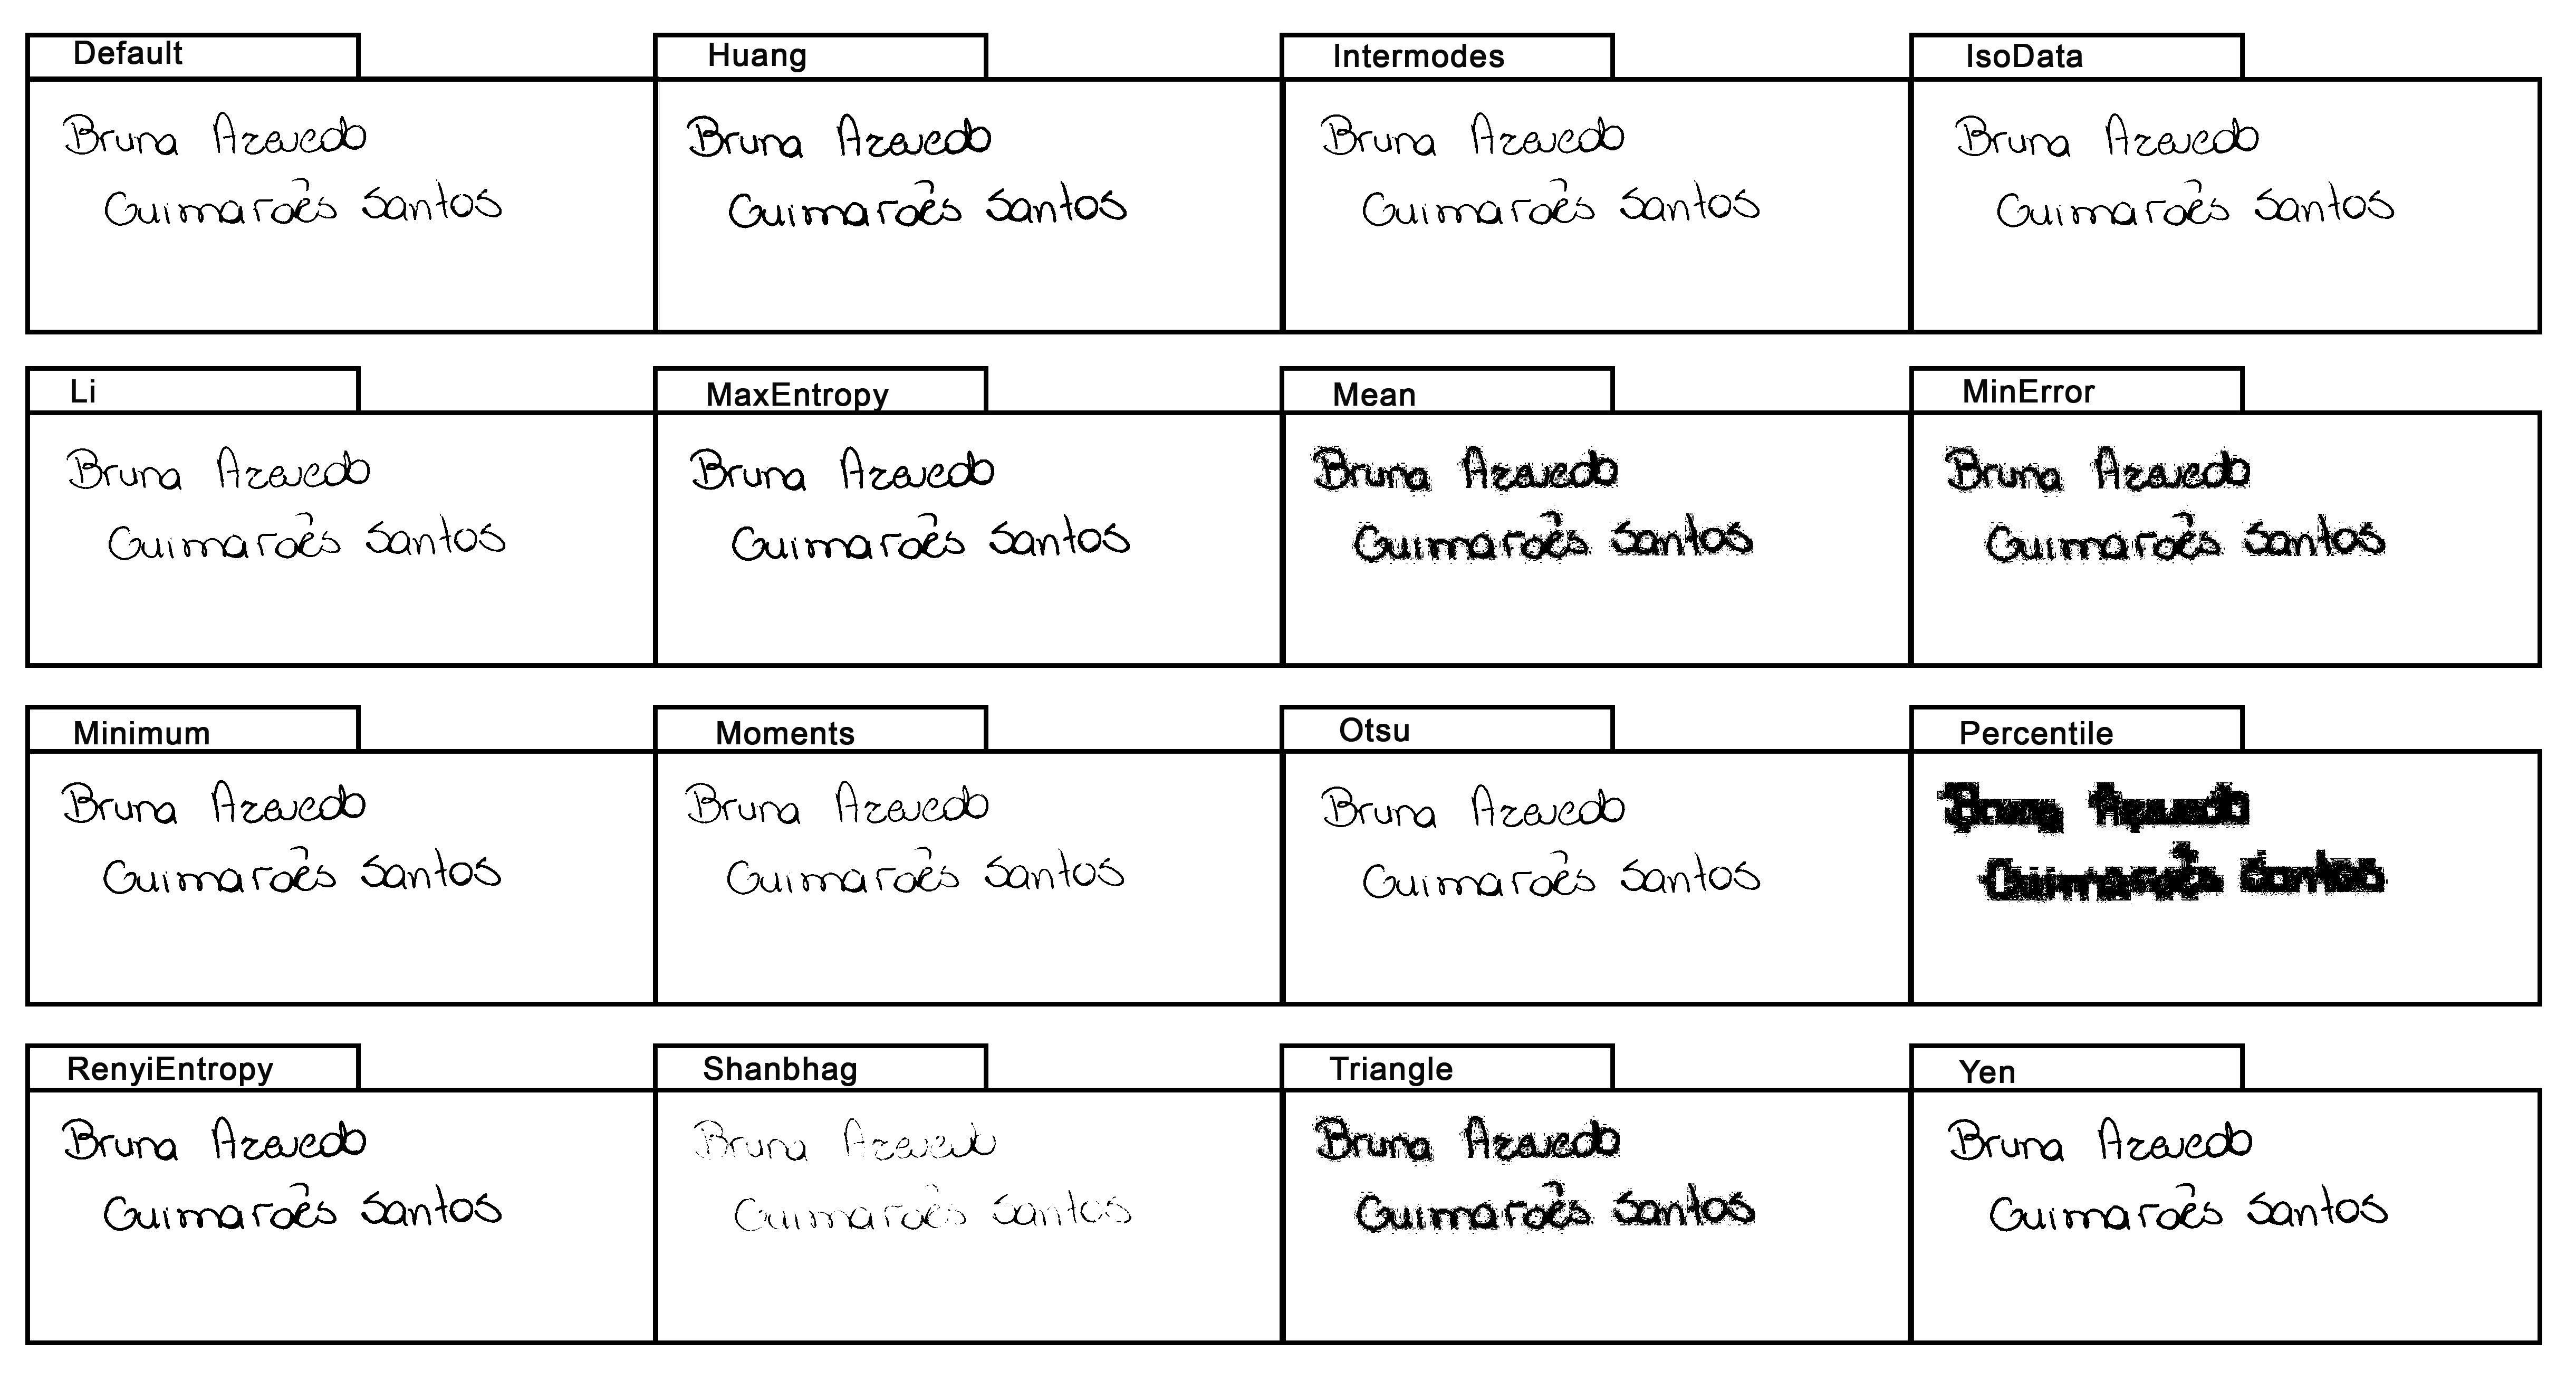
\includegraphics[scale= 0.09]{Met_threshold.jpg}
				\caption{Métodos de limiarização}
				\label{fig:metodos}
			\end{figure}
			\subsubsection{Default}
				Este é o método original de limiar automático disponível no ImageJ, que é uma variação do algoritmo IsoData.
			\subsubsection{Moments}
				O método de Moments tenta preservar os momentos da imagem original no resultado com limite. Os valores de limiar são calculados de forma determinística de tal forma que os momentos de uma imagem de entrada são preservados na imagem de saída. Resultados experimentais mostram que a abordagem pode ser empregada para limitar uma determinada imagem a classes significativas de nível de cinza\textsuperscript{\cite{eliceiri2017}}.
			\subsubsection{Percentile}
				Necessária para o reconhecimento de padrões semelhança-invariante\textsuperscript{\cite{doyle1962}}, em que presume-se uma fração de pixels do primeiro plano seja 0,5\textsuperscript{\cite{eliceiri2017}}.
				Todos os métodos apresentados foram necessários para o tratamento e segmentação das assinaturas para que o resultado final baseado em um arquivo compatível com o programa \textit{Weka}, gerando atributos válidos no arquivo resultante dos processos, para o aprendizado de máquina.
		\subsection{Treinamento}
			A etapa de treinamento foi realizada no programa Weka, onde foram assimilados arquivos arff do processamento realizado na seção de metodologia. Assim os resultado de aprendizado de máquina e testes serão apresentados nos três tipos de limiarização aplicados.
		
	\section{Resultados}
		As tabelas seguir são apresentados os resultados obtidos com os treinamentos e testes citados anteriormente. De forma geral, os resultados foram positivos, ao verificar se, com base nos dados de treinamento, as assinaturas de teste pertenciam ao mesmo autor. A primeira coluna demonstra o número de instâncias utilizadas para treinamento, e as demais, o número de instâncias utilizadas para testes e o respectivo resultado da classificação, utilizando o algoritmo \textit{Random Forest}:
		
		\begin{table}[ht]
			\centering
			\caption{Comparação de métodos assinatura Bruna}
			\label{tab:ComparacaoBruna}
			\begin{tabular}{ p{3cm}|c|c|c|c }
				\hline
				Método & Treinamento & Primeiro teste & Segundo teste & Terceiro teste\\
				\hline
				\multirow{1}{1cm}{Default}  & 59743 (100\%) & 16021 (100\%) & 16216 (100\%) & 15360 (100\%)\\
				\hline
				\multirow{1}{1cm}{Moments} & 55493 (100\%) & 15136 (100\%) & 15183 (100\%) & 14272 (100\%) \\
				\hline
				\multirow{1}{1cm}{Percentile} & 274108 (100\%) & 69968 (100\%) & 73433 (100\%) & 69579 (100\%) \\
			\end{tabular}
		\end{table}

		\begin{table}[ht]
			\centering
			\caption{Comparação de métodos assinatura Kênia}
			\label{tab:ComparacaoKenia}
			\begin{tabular}{ p{3cm}|c|c|c|c }
				\hline
				Método & Treinamento & Primeiro teste & Segundo teste & Terceiro teste\\
				\hline
				\multirow{1}{1cm}{Default}  & 38487 (100\%) & 9840 (100\%) & 11138 (100\%) & 9774 (100\%)\\
				\hline
				\multirow{1}{1cm}{Moments} & 36157 (100\%) & 10403 (100\%) & 10403 (100\%) & 9197 (100\%) \\
				\hline
				\multirow{1}{1cm}{Percentile} & 115075 (100\%) & 32409 (100\%) & 32409 (100\%) & 29128 (100\%) \\
			\end{tabular}
		\end{table}
	
		\begin{table}[ht]
			\centering
			\caption{Comparação de métodos assinatura Raoni}
			\label{tab:ComparacaoRaoni}
			\begin{tabular}{ p{3cm}|c|c|c|c }
				\hline
				Método & Treinamento & Primeiro teste & Segundo teste & Terceiro teste\\
				\hline
				\multirow{1}{1cm}{Default}  & 13519 (100\%) & 4073 (100\%) & 3130 (100\%) & 3896 (100\%)\\
				\hline
				\multirow{1}{1cm}{Moments} & 12575 (100\%) & 3930 (100\%) & 2944 (100\%) & 3701 (100\%) \\
				\hline
				\multirow{1}{1cm}{Percentile} & 75311 (100\%) & 19943 (100\%) & 16950 (100\%) & 21625 (100\%) \\
			\end{tabular}
		\end{table}
	
	\section{Conclusão}
		Com base na proposta do artigo, os resultados não foram satisfatórios, pelo motive de termos agregado uma comunidade de dados ínfima com base nos trabalhos relacionados, que em seus estados foram utilizados um volume considerável. Se é necessário um conjunto de computadores mais potentes, pelo fato do aprendizado consumir quase que totalmente a memória do computador, isso foi de grande impacto no desempenho e processamento dos testes e treinamento. Entretanto, com os resultados obtidos entendemos que a quantidade de dados para o aprendizado é primordial para o refinamento da precisão no aprendizado de máquina.

	\bibliographystyle{abnt-num}
	\bibliography{sbc-template}	
\end{document}
